\section{Indium Electroplating}

\subsection{Introduction}
There are a variety of methods for indium electroplating, while I did not select the electroplating process there are a variety of methods available that are commonly used in industry. The largest differences tend to be in what comprises the solution and the operating temperatures.

\subsection{Process}
The indium electroplating process is based on a now industry standard process that is known to yield good results while requiring a minimum of process optimization.

CITE THE INDIUM CORPORATION AND THE ADDITIVES IN THEIR ELECTROPLATING SOLUTION

IDENTIFY BENEFITS OF EACH CHEMICAL IN THE THING? IF POSSIBLE?

Adapting the indium electroplating process to the E3-3139 and the resources available there, the process was as follows:

\begin{center} % center the minipage
    \begin{framed} % add a border to the minipage
        \begin{minipage}{0.8\textwidth} % set the width of the minipage
            \raggedright % align the text to the left
            \textbf{Note}: Electroplating procedure used in the E3-3139 Lab

            \vspace{0.1cm} % add some vertical space between the title and the body of the minipage

            \mpsection{Purpose}
            Depositing Indium from an electroplating solution onto samples for die-bonding. The solution used is from Indium Corporation of America and uses their Indium Sulfamate Plating Kit to perform the Indium electroplating.

            \mpsection{Equipment}
            \begin{center}

            \begin{tabular}{|l|c|}
                \hline
                \textbf{Name}  &   \textbf{Quantity} \\
                \hline
                Fume Hood                           &	1 \\
                N2 Gun                              &	1 \\
                DI Water Bottle                     &	1 \\
                2L Beakers                          &	2 \\
                400mL Beaker                        &	1 \\
                200mL Beaker                        &	1 \\
                1L HDPE Bottle                      &	1 \\
                500mL HDPE Bottle                   &	1 \\
                Hotplate with Magnetic Stirring     &	1 \\
                Magnetic Stir Bar                   &   1 \\
                Funnel                              &	1 \\
                Insulated Copper Wire               &	2 \\
                Banana Plug Wires                   &	2 \\
                Copper Alligator Clips              &	2 \\
                Tweezers kit                        &	1 \\
                Custom Sample Holder                &	1 \\
                \hline
            \end{tabular}

            \vspace{0.5cm}

            \begin{tabular}{|l|c|}
                \hline
                \textbf{Name} & \textbf{Quantity} \\
                \hline
                Indium Sulfamate Plating Bath        & 1L \\
                Indium Anode (30cm x 2.5cm x 1.5mm)  & 1 \\
                Sulfamic Acid                        & 150mL \\
                15-20\% HCl                          & 150mL \\
                DI Water                             & 10L \\
                pH Paper Set or pH Meter             & 1 \\
                Clean Room Wipes Pack                & 1 \\
                \hline
            \end{tabular}

            \end{center}

        \end{minipage}
    \end{framed}
\end{center}


\begin{center} % center the minipage
    \begin{framed} % add a border to the minipage
        \begin{minipage}{0.8\textwidth} % set the width of the minipage
            \raggedright % align the text to the left
            \setcounter{mpsection}{2}

            \mpsection{Chemical Hazards}

            No new chemicals are being introduced into the lab, and the SDS of the chemicals relevant to the experiment are attached with the following SOP.

            \begin{itemize}
                \item Sulfamic Acid
                \item Indium Sulfamate Plating Bath
            \end{itemize}

            \mpsection{Safety Procedure}
            \begin{itemize}
                \item Lab apron, rubber gloves, safety goggles, face-shield, and closed-toed shoes must be worn before interacting with any chemicals
                \item To avoid spills ready all beakers and bottles under the fume-hood over clean room wipes before opening
                \item Use care when opening and pouring chemicals to avoid spills during the preparation and process of the experiment
                \item Do not touch your face or exposed skin during the process of the experiment
                \item Always wash hands after handling any chemicals or materials
                \item Avoid inhaling the mist or vapor of the chemicals, and avoid exposure to eyes and skin
                \item Perform the entire experiment under a fume hood
            \end{itemize}
        \end{minipage}
    \end{framed}
\end{center}


\begin{center} % center the minipage
    \begin{framed} % add a border to the minipage
        \begin{minipage}{0.8\textwidth} % set the width of the minipage
            \raggedright % align the text to the left
            \setcounter{mpsection}{4}
            \mpsection{Process Flow}
            \begin{enumerate}
                \item Prepare the fume hood surface:
                \begin{enumerate}
                    \item Place clean room wipes on the surface of the fume hood.
                    \item Ensure your name and contact information are visible at the work location in case people need to contact you.
                    \item Chemicals in the beakers should be identified and all beakers should be labeled with what chemicals will be in them.
                \end{enumerate}
                \item Place the digital hotplate with stirring functionality inside the fume hood.
                \begin{enumerate}
                    \item Do not place a wipe on the hotplate surface. This interferes with the transmission of heat to the beaker and its contents. It may also present a fire hazard. This is regardless of weather the heating element will be used.
                    \item Do NOT turn on the heating element over the course of this experiment.
                \end{enumerate}
                \item Set all four beakers (2x 2L, 1x 400mL, 1x 200mL) under the fume hood, and set one 2L beaker on the hotplate. Place the stir bar inside the beaker on the hotplate.
                \item Build the Custom Sample Holder and place in the beaker on the hotplate at the appropriate distance for the electroplating process (~5cm).
                \item Place the indium anode into the beaker on the hotplate, ensure that there is an appropriate distance from the sample and ensure that the electrode is connected to an alligator clip. Be sure to use fresh gloves when handling the indium electrode to avoid contamination.
                \begin{enumerate}
                    \item Anode/cathode distance may alter grain size and uniformity of electroplating.
                    \item It is essential that the sample is perpendicular to the normal of the anode (indium)
                \end{enumerate}

                \item Ensure that all PPE is worn appropriately, and no skin is exposed.
                \item Acquire the indium sulfamate solution, sulfamic acid, and diluted HCl solutions from the Acids cabinet and transport it to the fume hood.
                \begin{enumerate}
                    \item Pour the indium sulfamate solution into the beaker on the hotplate.


                    \textit{Ensure that the hotplate is OFF and the beaker is at room temperature to avoid shattering glass}
                    \item Pour the sulfamic acid into the 200mL beaker
                    \item Pour the HCl dilution into the 400mL beaker
                    \item Pour ~2L of DI water into the remaining large beaker
                    \item Turn on stirring to ~300RPM
                \end{enumerate}

                \item Check the pH of the indium sulfamate solution and verify it is between 1.5 and 2. If the pH exceeds 2 titrate sulfamic acid and mix until the pH enters the range again.
                \begin{enumerate}
                    \item Titration of sulfamic acid into the indium sulfamate solution can be done using a pipette that is labeled and only to be used for sulfamic acid. Since the exact pH is not important titration with a pipette is sufficient and a buret is not required.
                    \item Note that all tools used in the titration process must be rinsed with DI water and dried with N2.
                \end{enumerate}
            \end{enumerate}
        \end{minipage}
    \end{framed}
\end{center}


\begin{center} % center the minipage
    \begin{framed} % add a border to the minipage
        \begin{minipage}{0.8\textwidth} % set the width of the minipage
        \raggedright % align the text to the left

        \begin{enumerate}
            \setcounter{enumi}{8}
            \item Power should ideally be supplied with a pulsed constant current source and set to values in accordance with current over the plating surface area.
            \begin{enumerate}
                \item Ensure that the power supply is set and ready but disconnected from the sample now.
                \item Measure the surface area of the sample and validate that current supplied to the sample is nominal to $10-20A/ft^2$ or $0.01-0.02A/cm^2$. For the current design this corresponds to nominal values of (0.02A, 0.1V)
                \item Power should be connected as NEGATIVE terminal to sample and POSITVE terminal to indium anode
                \item Electroplating time is a function of the current density and expected final thickness of the deposited indium.
            \end{enumerate}

            \item Rinse the sample with DI water, place into HCl solution for the activation time (~5min), rinse again with DI water, and place into the sulfamic acid solution for cleansing (~3min).
            \begin{enumerate}
                \item The sample should be attached to the custom holder
                \item The HCl solution is required for cleaning and acid-activation (see the guide to indium plating).
                \item The sulfamic acid ensures the pH of the base metallization surface remains acidic and no reformation of oxide occurs.
            \end{enumerate}

            \item Place the sample into the plating bath at the appropriate distance and turn on the power supply for the target plating time.
            \begin{itemize}
                \item See the Indium electroplating guide for more information on how this affects the grain size
            \end{itemize}
        \end{enumerate}

        \vspace{0.5cm} % add some vertical space between the body of the minipage and the closing statement

        \textit{-- Waste disposal, storage instructions for equipment and materials, emergency procedures, and MSDS can be found in the original electroplating SOP document. They were not attached for brevity }

        \end{minipage}
    \end{framed}
\end{center}


The process used here allows us to electroplate indium onto the substrate that is Chrome-Gold on Sapphire. Both chromium and gold are excellent materials for indium to easily electroplate onto.
% TODO PROVIDE CITATION

\newpage

\subsection{Existing Setup Description}

In summary the process has us prepare the sample with acids before placing into the plating solution. Then the sample holder and sample are submerged in the plating solution and the current source is applied. However, due to cost constraints a voltage source was obtained to perform in place of a current source.

\begin{wrapfigure}{L}{0.25\textwidth}
    \centering
    \includegraphics[width=0.25\textwidth, angle=90]{Main/Ch1/Aligator_clip.jpeg}
    \caption{\raggedright Image of the flat mouth alligator clip used to clamp onto the sample}
\end{wrapfigure}

A current source would have been preferred over a voltage source due to several reasons. Since electroplating is a process where metal ions are deposited on a substrate through the use of an electric current. The amount of metal deposited is directly proportional to the amount of electric charge that flows through the system, which means that controlling the current is crucial for controlling the thickness and quality of the plated layer.

With a current source, the current can be precisely controlled and maintained at a constant level, which results in consistent and uniform plating as a function of time. On the other hand, a voltage source may not provide a consistent current, as the resistance of the plating solution can vary due to factors such as temperature or impurities, leading to poor plating results.


\begin{wrapfigure}{R}{0.25\textwidth}
    \centering
    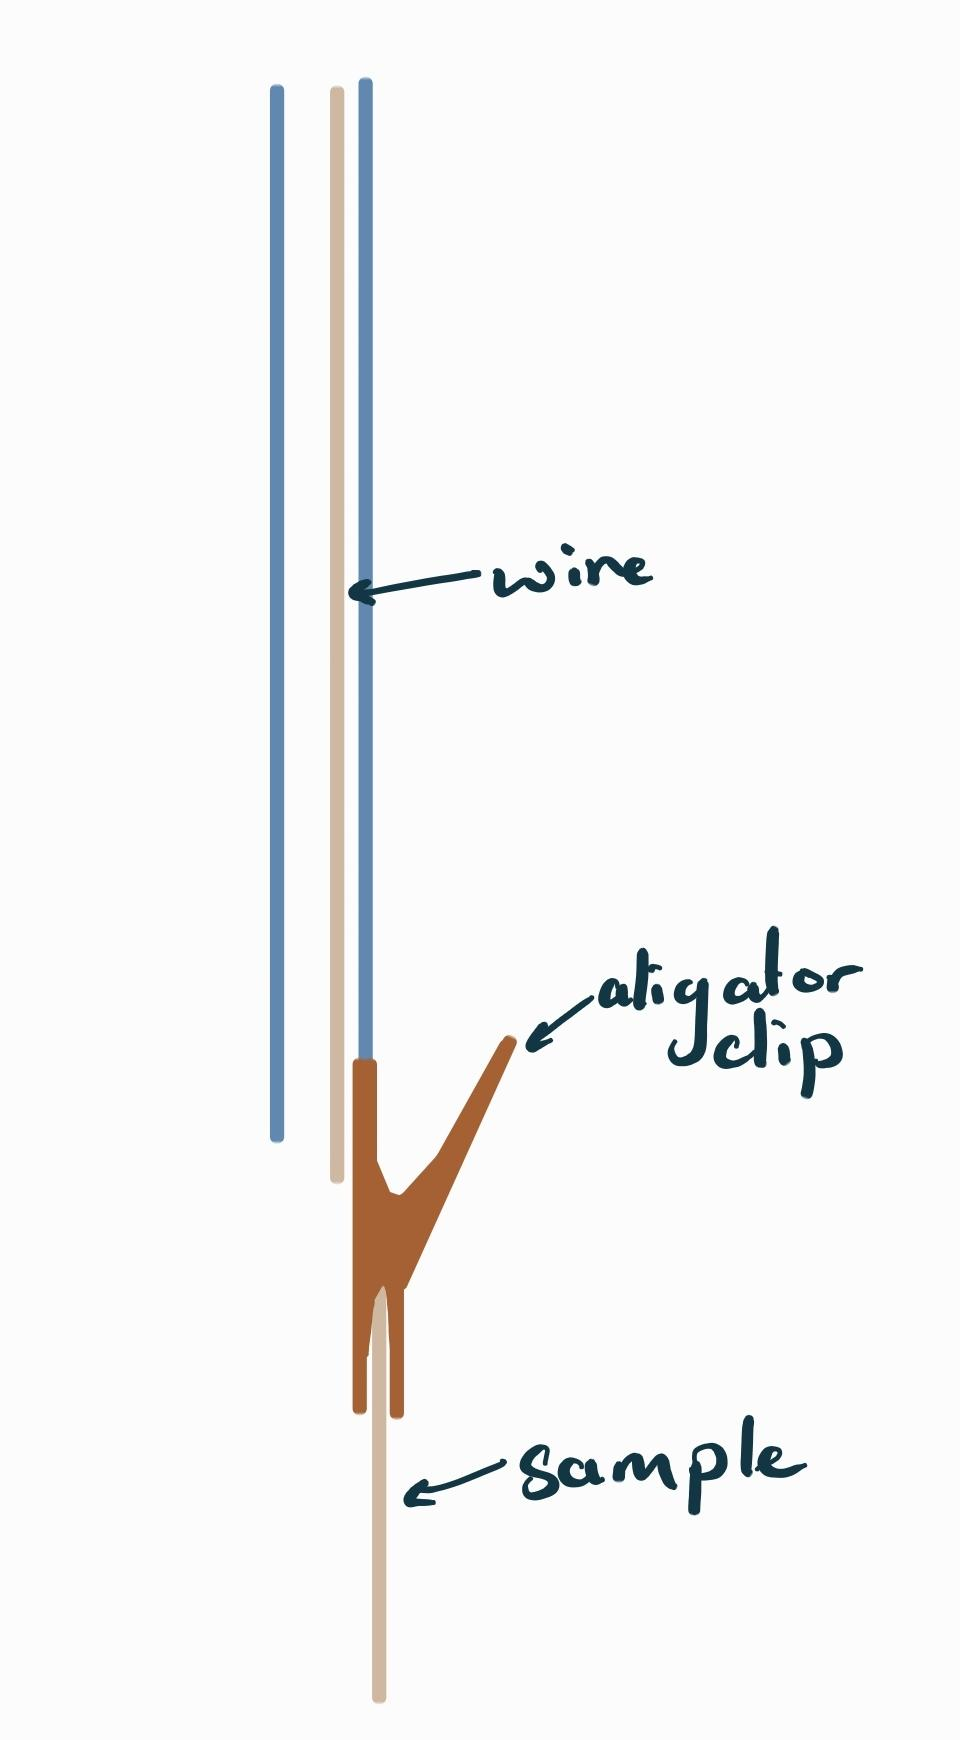
\includegraphics[width=0.25\textwidth]{Main/Ch1/Current Sample holder.png}
    \caption{Line drawing of the aligator clip and sample }
\end{wrapfigure}

Another advantage of using a current source is that it allows for better control over the plating process and reduces the risk of over-plating or under-plating. With a voltage source, the voltage applied to the system can cause the plating rate to fluctuate, which can result in uneven thickness or even damage to the substrate. In contrast, a current source ensures a constant and controlled deposition rate, which minimizes the risk of defects or damage to the substrate.

Using a voltage source with an ammeter can be equivalent to a current source in certain situations. This is because the voltage applied to a circuit is directly proportional to the current flowing through it. By measuring the current in the circuit using an ammeter, the current can be controlled by adjusting the voltage. In this way, the voltage source with an ammeter can effectively act as a current source.


\begin{wrapfigure}{L}{0.25\textwidth}
    \centering
    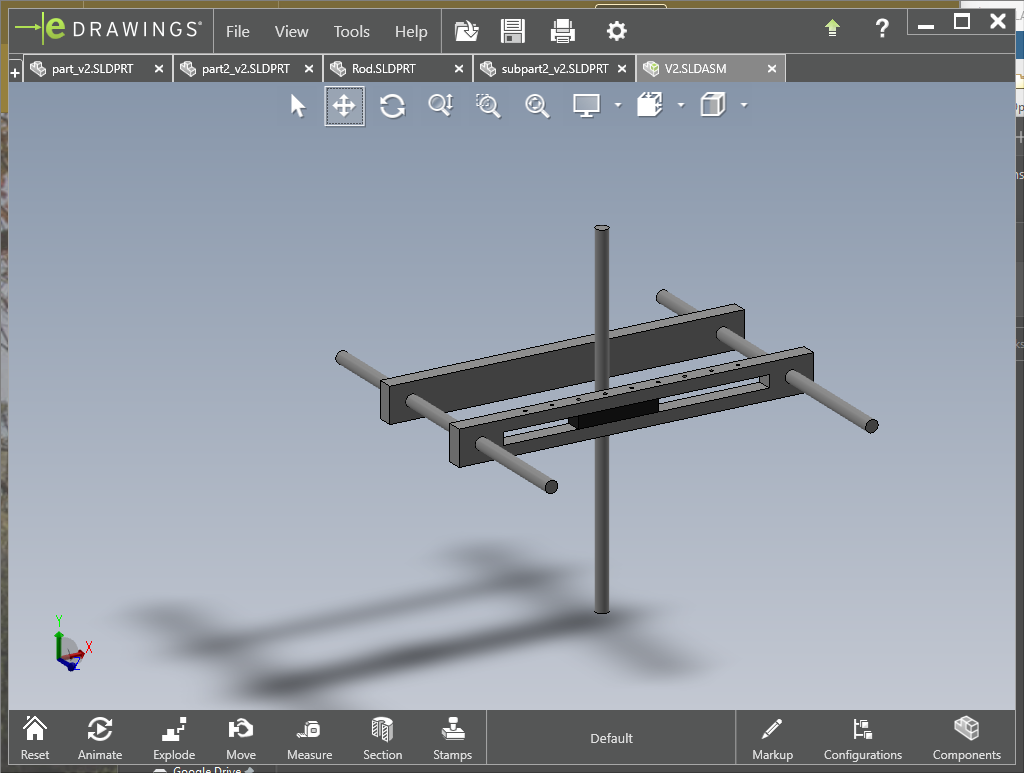
\includegraphics[width=0.25\textwidth]{Main/Ch1/Sample_holder.png}
    \caption{3D Rendering of the sample holder}
\end{wrapfigure}

The sample holder consists of two plastic blocks that are held together by two steel bars. Thumbscrews are used to lock the relative position of the plastic pieces in place while the assembly 'floats'  on the lip of the beaker the sample is submerged into. One of the two plastic pieces has a stopper that helps constrain the position of the assembly on the beaker while the other plastic piece holds the glass rod and alligator clip.

The glass rod is attached to the plastic piece and has the alligator clip on it. The clip and corresponding cathode holder are wrapped in a PTFE sleeve that helps minimize stray electric fields and electroplating onto the cathode wire.



\subsection{Phsyiscal Problems with the setup}

% TODO Replace with SI units instead of mA ...
% TODO Replace derivative with derivative library maybe?
The existing setup came with an analog voltage supply that was only able to provide analog control of the voltage based on two knobs (a fine and coarse). This control was only fine enough to $\pm 10mV$ where the derivative of the current with respect to voltage in the relevant regime was $\frac{d mA}{d mV} = \frac{0.3 mA}{1 mV}$.
This meant there was poor resolution on the current control with the previous power-supply with a current resolution of $\pm 3 mA$ which would be an insufficient resolution for the small area that was being plated.

I replaced the existing voltage supply with a Tektronics function generator as it provided an appropriate resolution and dynamic range for such the task.
The function generator would allow for pulsed plating as recommended by the indium corporation \cite{indiumCorpGrainStructure}

\subsection{Experimental Issues - Deviation from Theory}

According to the Indium corporation docs, the recommended electroplating current density for plating is \dots
Converting to SI units from ASME units we see that this yields a plating current of \dots . However in this analysis we have only considered the active plating area of the sample, and we have failed to consider the plating area of the exposed alligator clip that holds the sample.

The extra exposed area guarantees an incorrect characterization of the plating growth proportional to the exposed area for the indium bumps. We can show this simply from the following

\begin{equation}\tag{A}
    \begin{split}
        V &= I R \\
        I_{Plating} &= \frac{\text{Some fixed current}}{\text{Plating area}}  = J_{Plating} \times A_{Plating} \\
        V_{Plating} &= \text{Variable to satisfy plating current} \\
        R_{Total} &= R_{Anode} + R_{Plating Solution} + R_{Cathode} + R_{Wires} \\
        I_{Plating} &= s
    \end{split}
\end{equation}



HERE I WANT TO IDENTIFY THE PLATING GROWTH PPER SECOND AS A FUNCTION OF THE PLATING AREA

DESIGN OF ALIGATOR CLIP WAS MESSING WITH OUR RESILTS

ACCOUNTINF FOR THE AREA OF THE ALIGATOR CLOP

DERIVING THE ARE OF THE ALGATOR CLOP BASED ON EXPECTED PLATING GROWTH RATE



\subsection{Development of a Repeatable Process}

TO DEVELOP A REPEATABLE PROCESS PICKING A DISTANCE AND ENSURING ALIGNEMENT

SELECTING A BETTER VOLTAGE SOURCE/CURRENT SOURCE MILLIVOLT CONTROL, RESOLUTION OF 0.02mA per milli Volt

